% Created 2017-02-10 ven. 11:27
% Intended LaTeX compiler: pdflatex
\documentclass[bigger]{beamer}
\usepackage[utf8]{inputenc}
\usepackage[T1]{fontenc}
\usepackage{graphicx}
\usepackage{grffile}
\usepackage{longtable}
\usepackage{wrapfig}
\usepackage{rotating}
\usepackage[normalem]{ulem}
\usepackage{amsmath}
\usepackage{textcomp}
\usepackage{amssymb}
\usepackage{capt-of}
\usepackage{hyperref}
\usetheme{Boadilla}
\author{Christophe Goudet}
\date{\today}
\title{}
\beamertemplatenavigationsymbolsempty
\usepackage{appendixnumberbeamer}
\hypersetup{
 pdfauthor={Christophe Goudet},
 pdftitle={},
 pdfkeywords={},
 pdfsubject={},
 pdfcreator={Emacs 24.5.1 (Org mode 9.0.4)},
 pdflang={English}}
\begin{document}


\section{Correlation model}
\label{sec:org958366e}
\begin{frame}[label={sec:org44f2794}]{Merging in \(\eta\)}
Two models of merging of the FULL (84NP) model are tested.
In both cases it relies on recorrelating \(\eta\) bins of some systematics.

\vfill

\begin{columns}
\begin{column}{0.5\columnwidth}
\alert{FullMerged}

Merge some systematics into Barrel+encap (48NP)
\begin{itemize}
\item MATCALO
\item MATCRYO
\item S12
\item PS
\end{itemize}
\end{column}

\begin{column}{0.5\columnwidth}
\alert{MergeEta}

Correlate all systematics in \(\eta\) (31NP)
\end{column}
\end{columns}
\end{frame}

\begin{frame}[label={sec:org6c8e211}]{Results}
\begin{columns}
\begin{column}{0.45\columnwidth}
\begin{center}
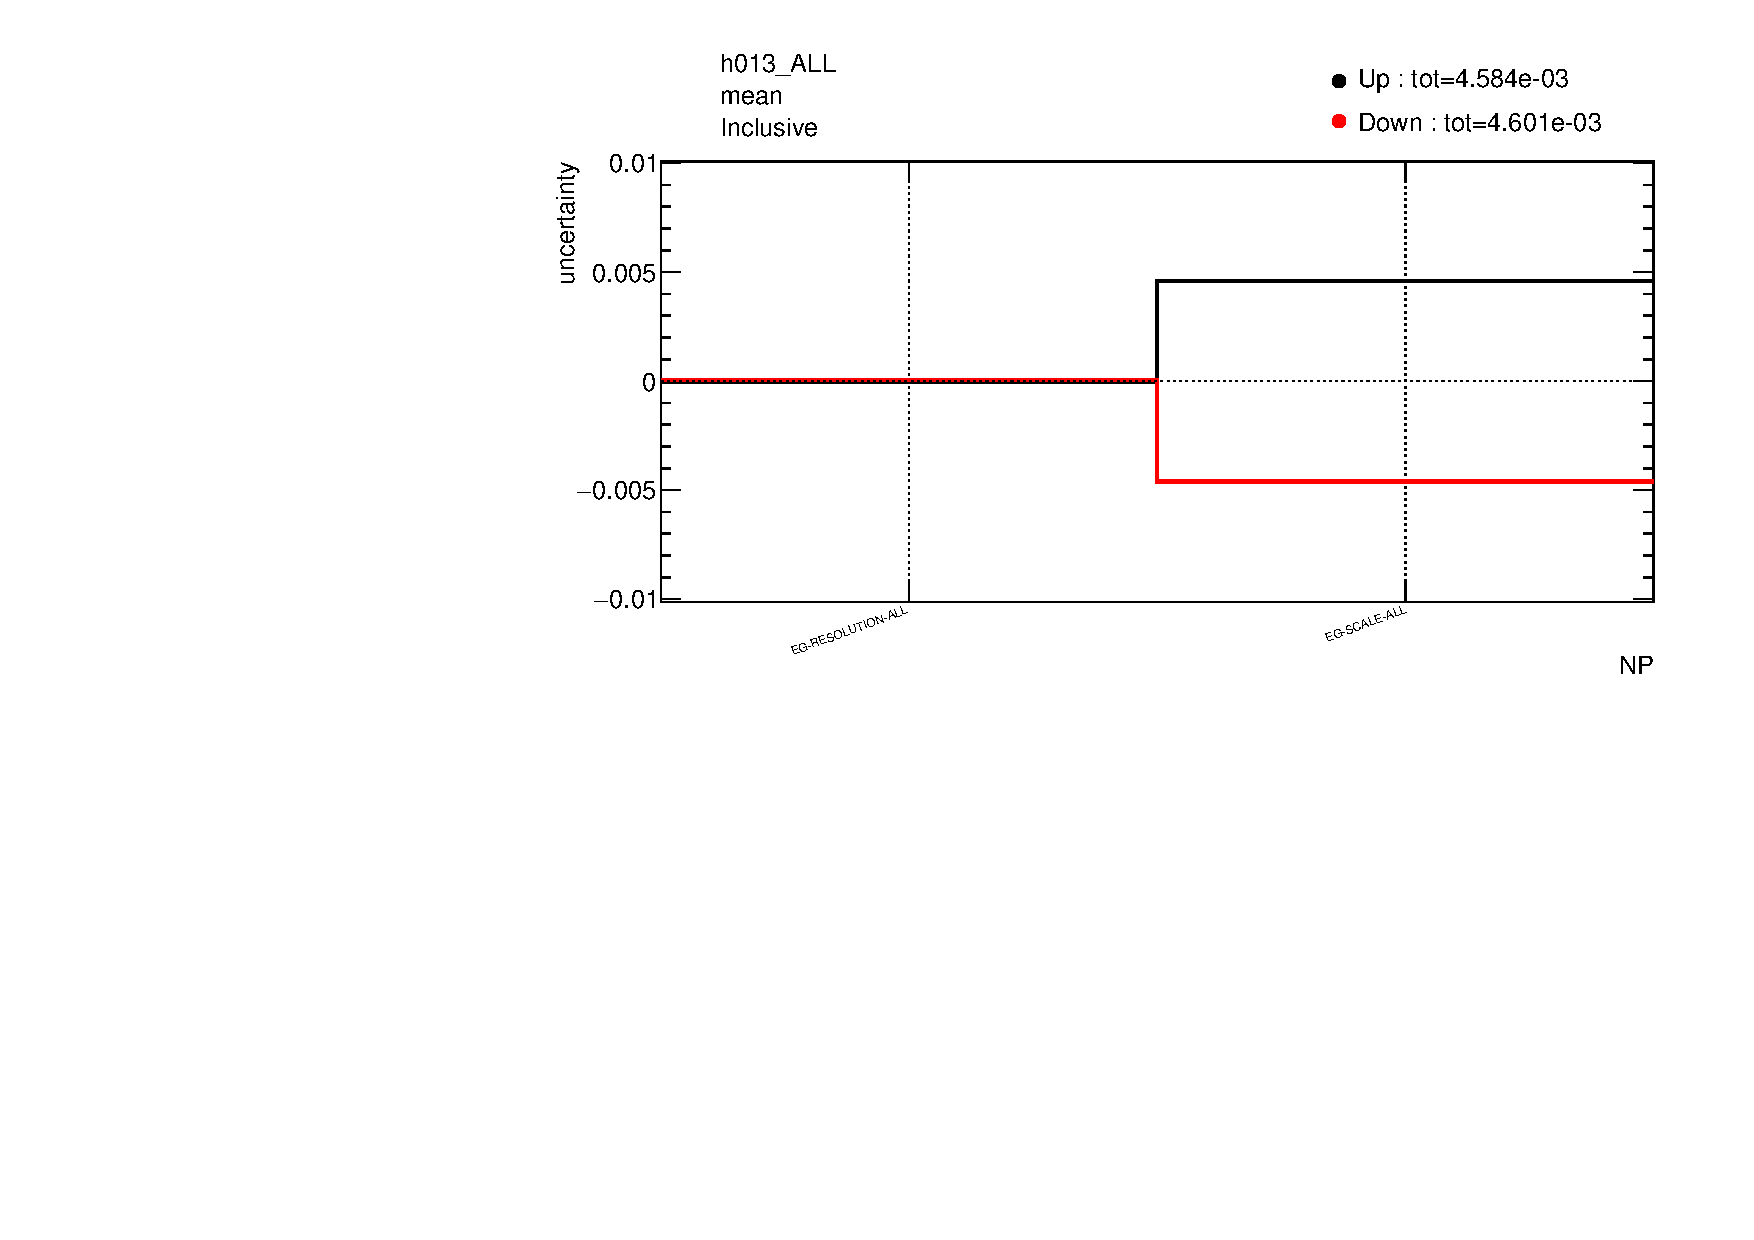
\includegraphics[width=\linewidth]{./plots/h013_ALL_Systematics_Inclusive_mean_mean.pdf}
\end{center}
\end{column}

\begin{column}{0.45\columnwidth}
\begin{center}
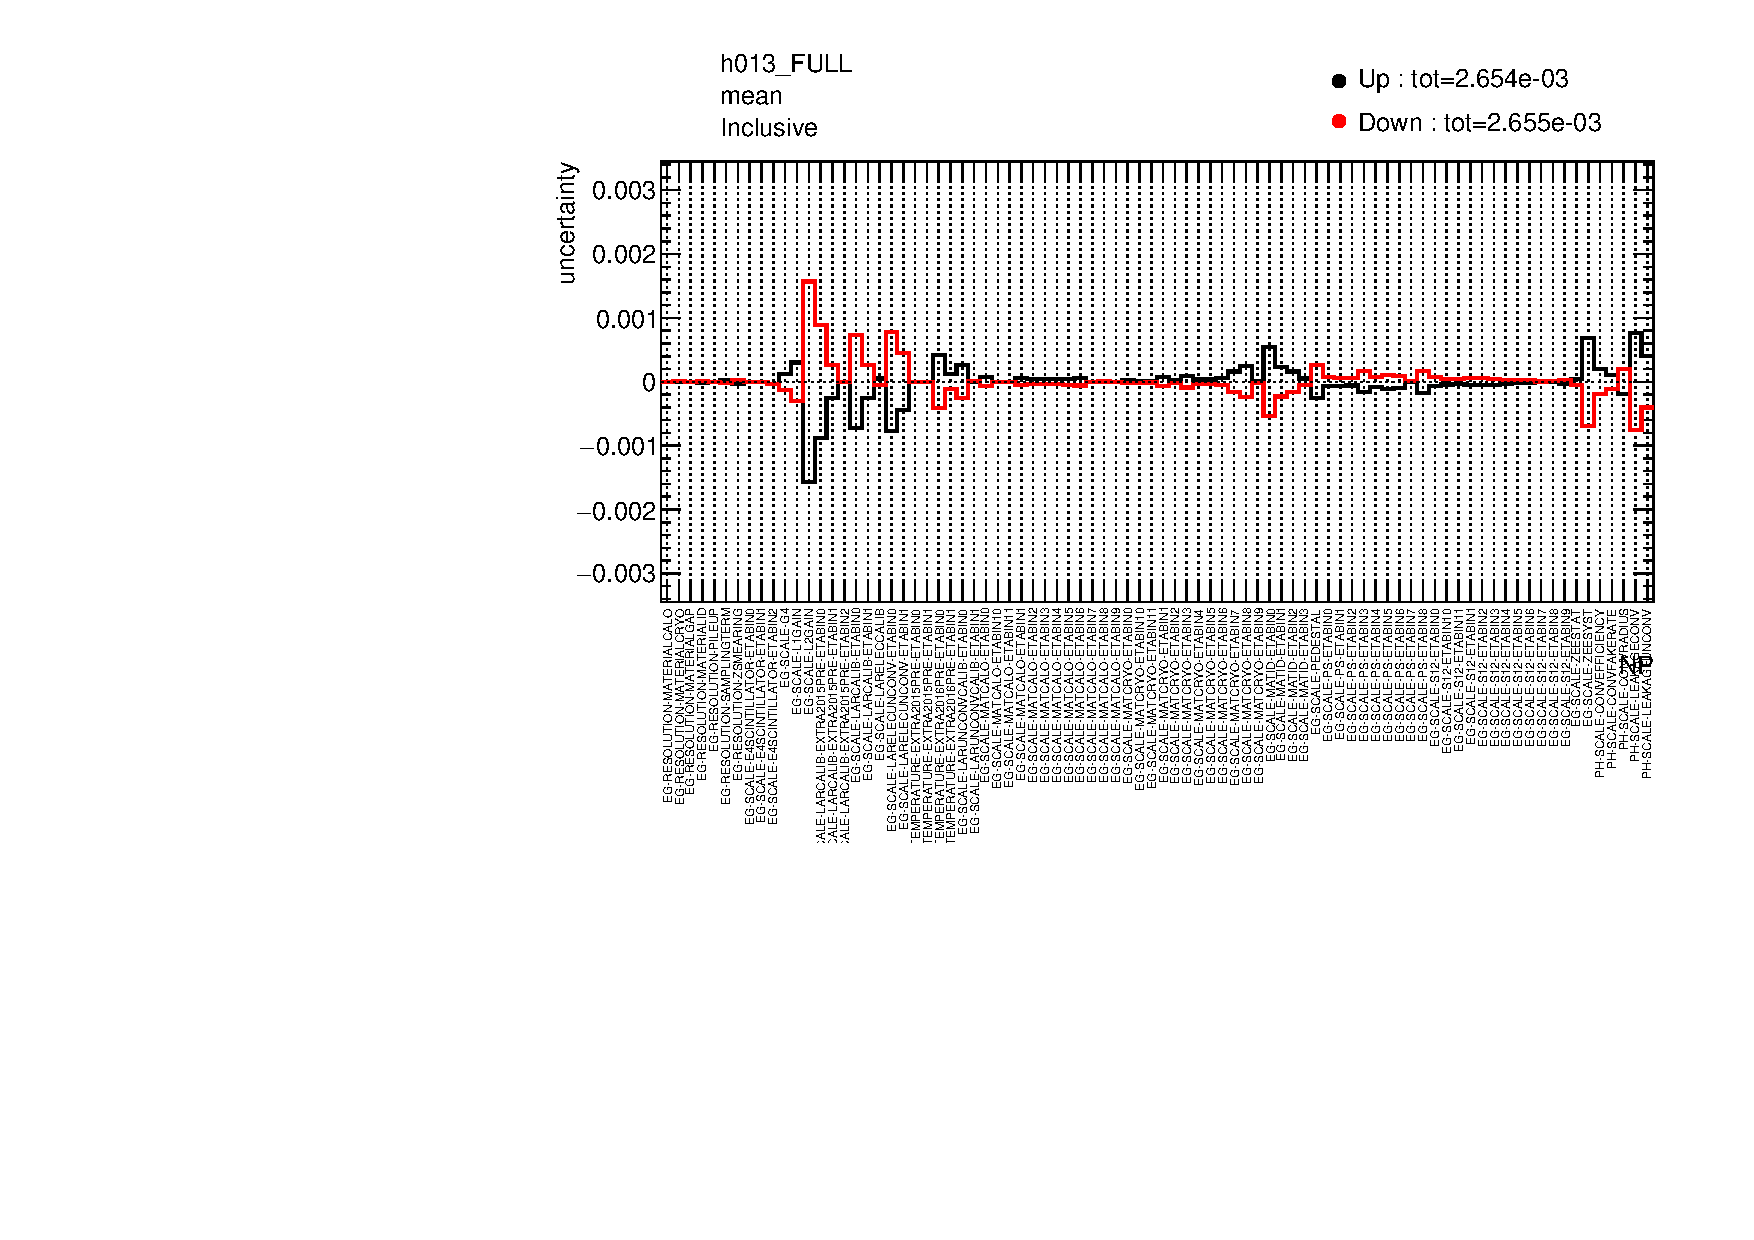
\includegraphics[width=\linewidth]{./plots/h013_FULL_Systematics_Inclusive_mean_mean.pdf}
\end{center}
\end{column}
\end{columns}

\begin{columns}
\begin{column}{0.45\columnwidth}
\begin{center}
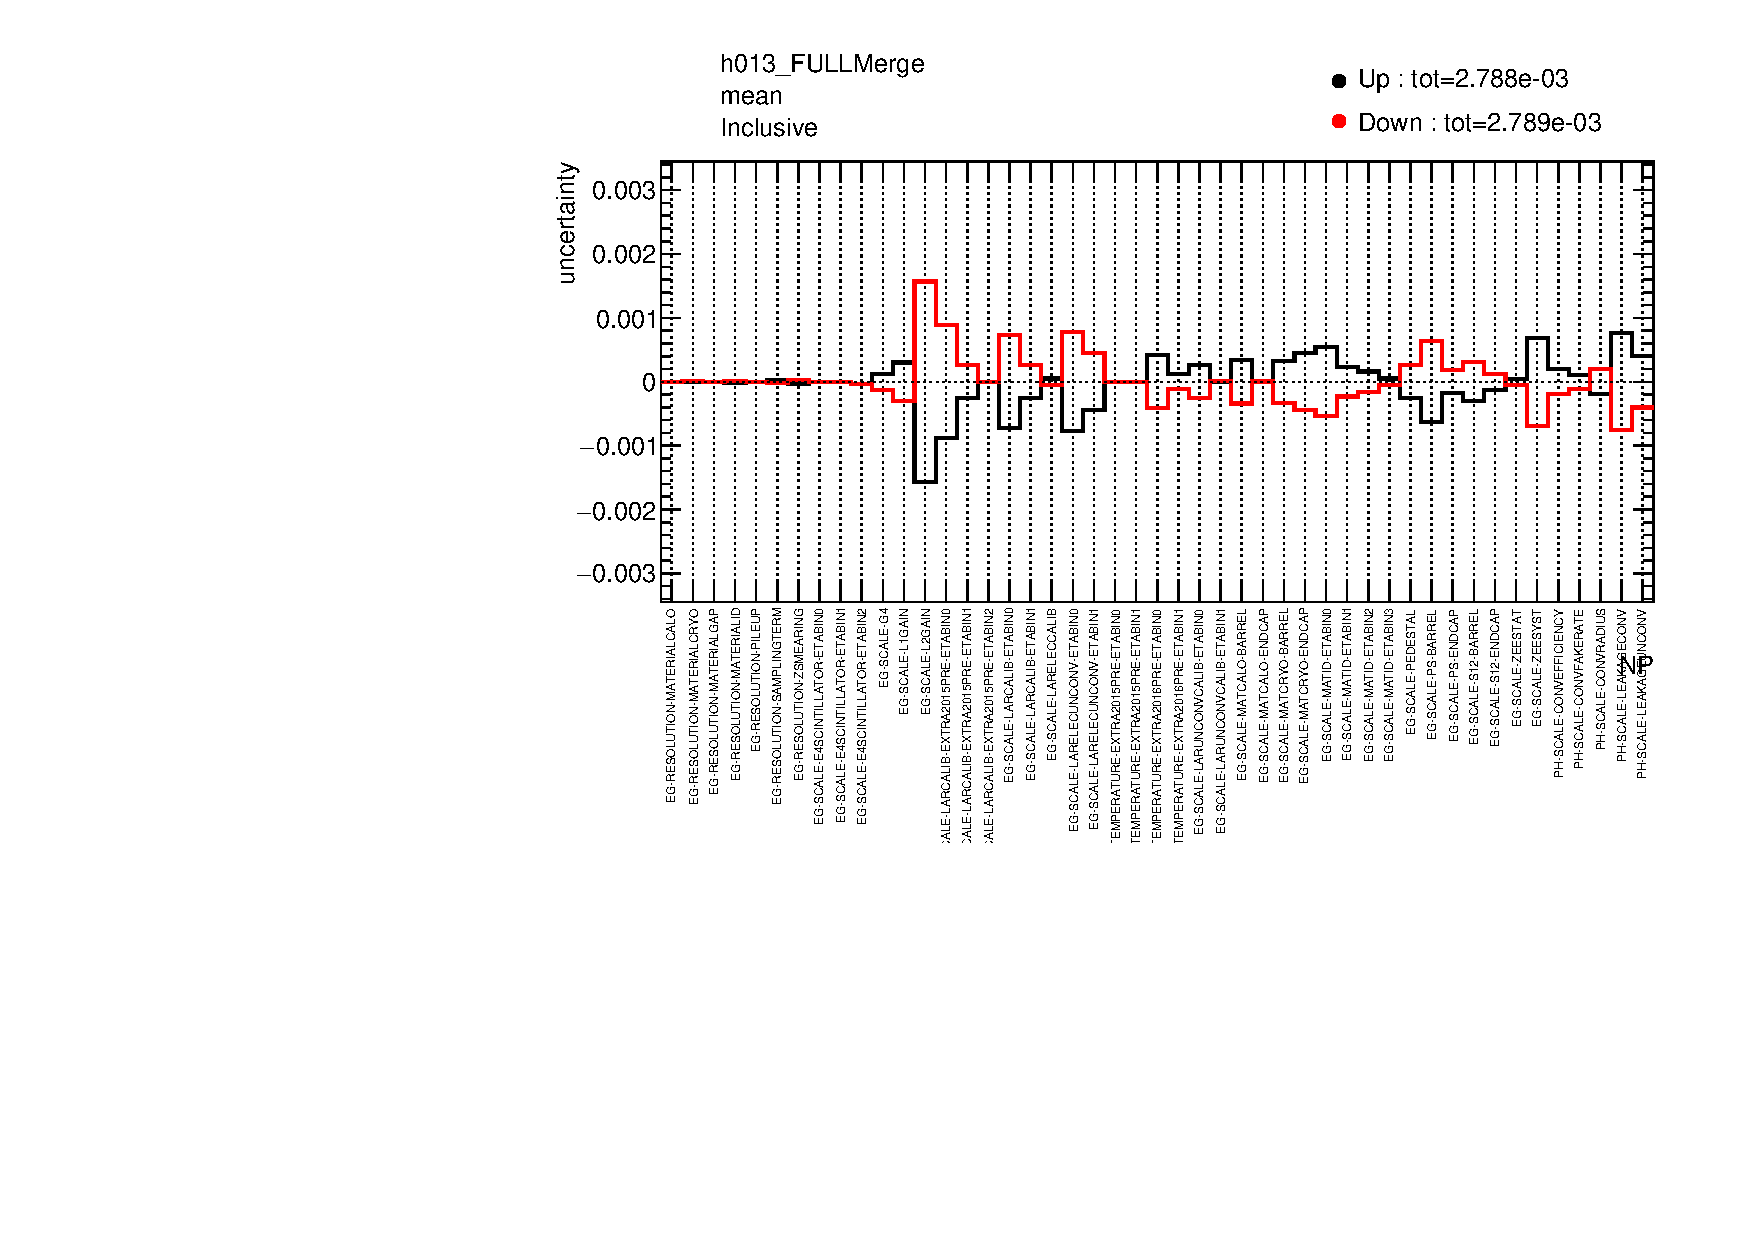
\includegraphics[width=\linewidth]{./plots/h013_FULLMerge_Systematics_Inclusive_mean_mean.pdf}
\end{center}
\end{column}

\begin{column}{0.45\columnwidth}
\begin{center}
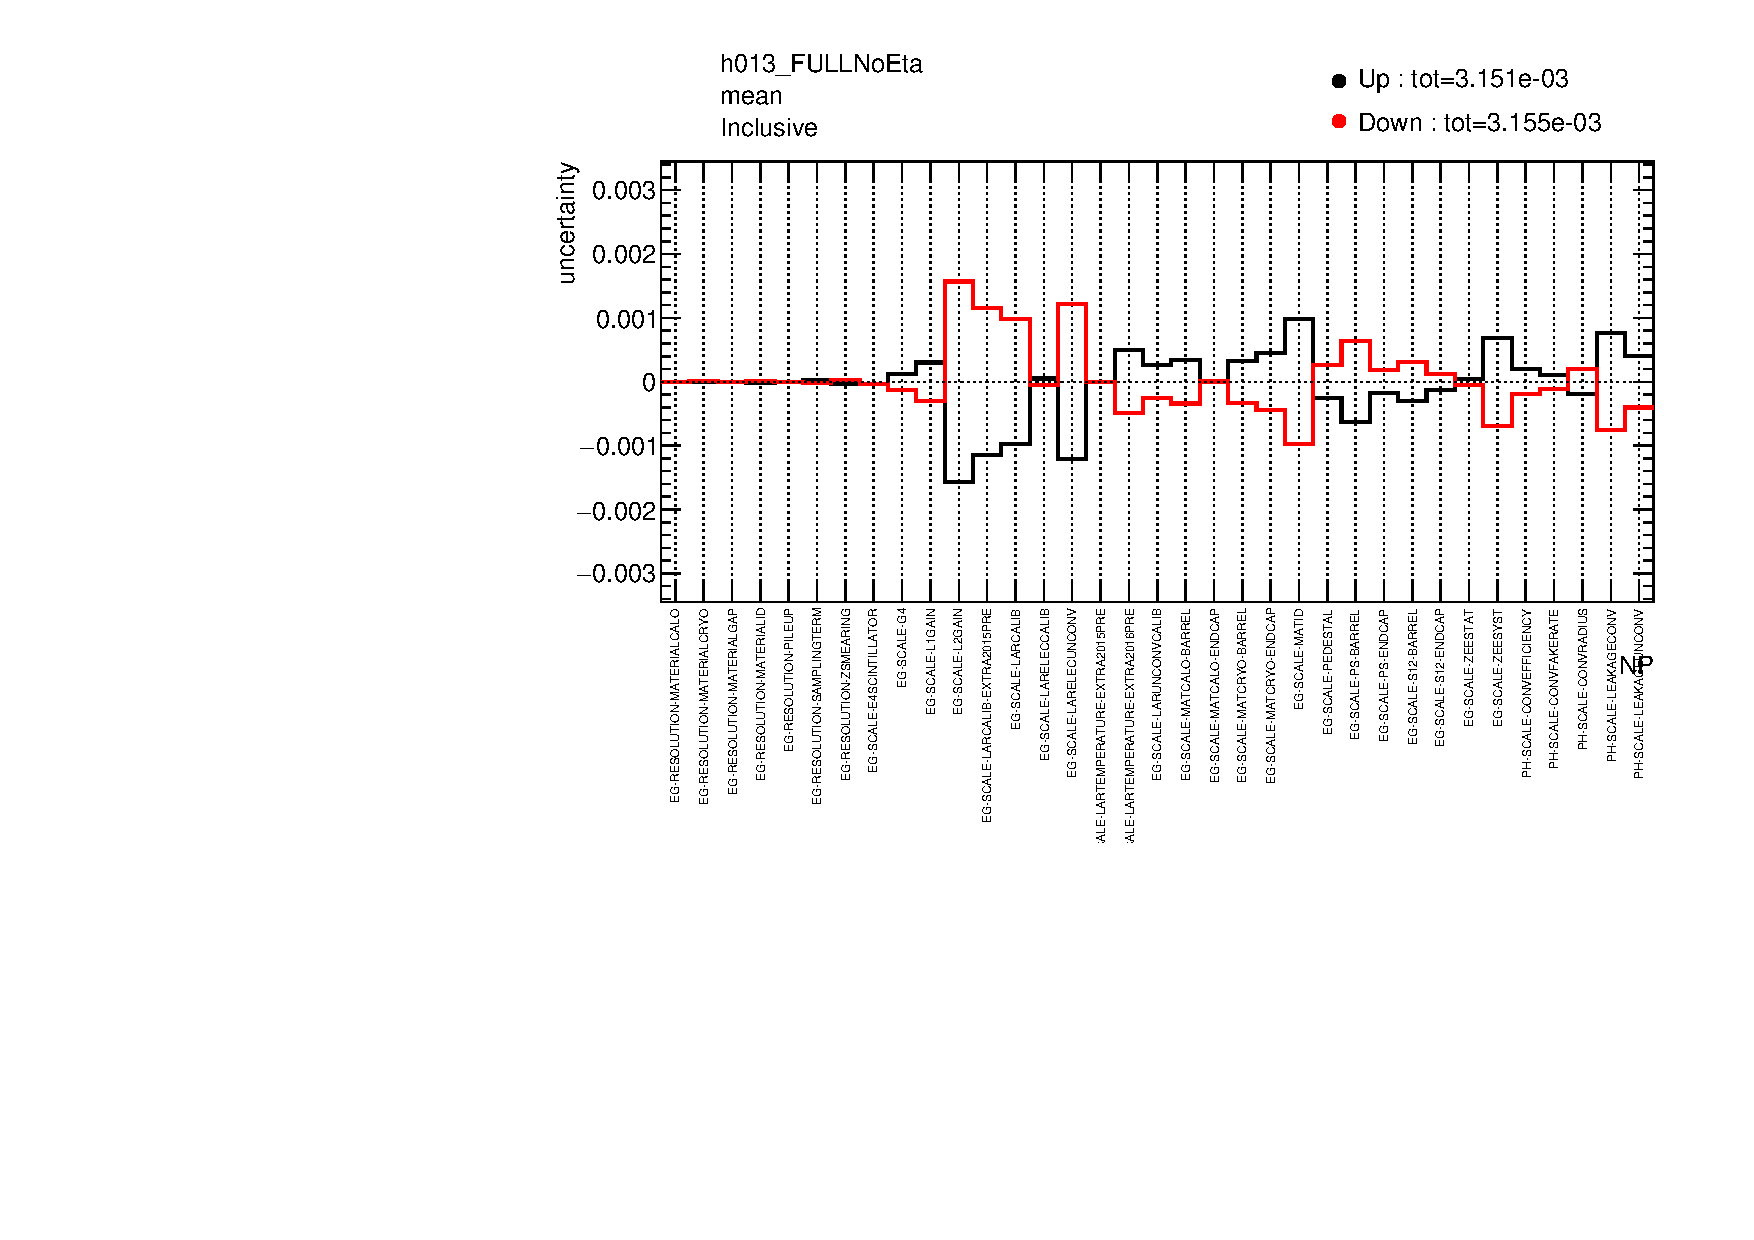
\includegraphics[width=\linewidth]{./plots/h013_FULLNoEta_Systematics_Inclusive_mean_mean.pdf}
\end{center}
\end{column}
\end{columns}
\end{frame}

\begin{frame}[label={sec:org0af9940}]{Comparison}
\begin{center}
\includegraphics[width=.9\linewidth]{/home/goudet/Documents/LAL/Zim/Hgam/PhotonSystematic/170209_CompareSystModel_h013.pdf}
\end{center}
\end{frame}
\section{h014}
\label{sec:org25b2903}
\begin{frame}[label={sec:orgc589fb6}]{ALL}
\begin{columns}
\begin{column}{0.5\columnwidth}
\begin{center}
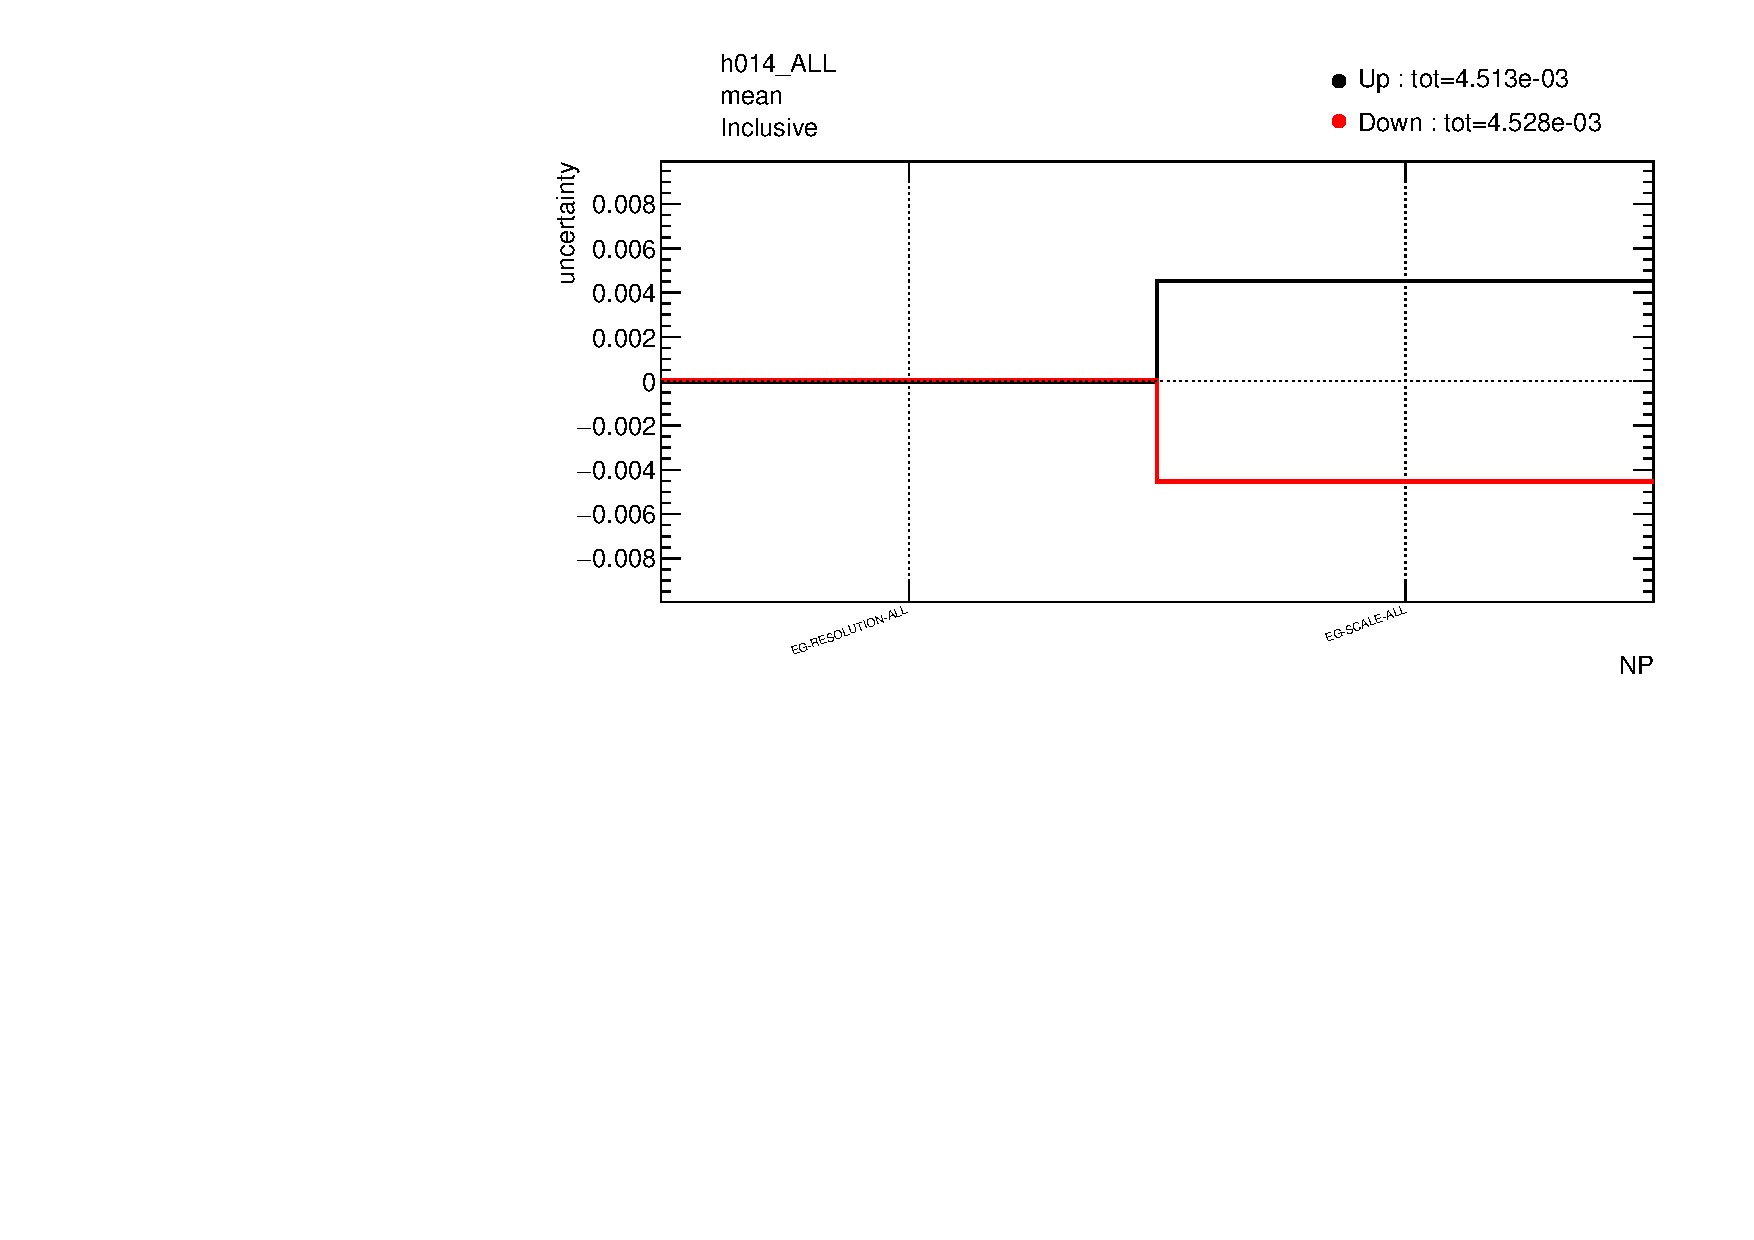
\includegraphics[width=\linewidth]{./plots/h014_ALL_Systematics_Inclusive_mean_mean.pdf}
\end{center}
\begin{center}
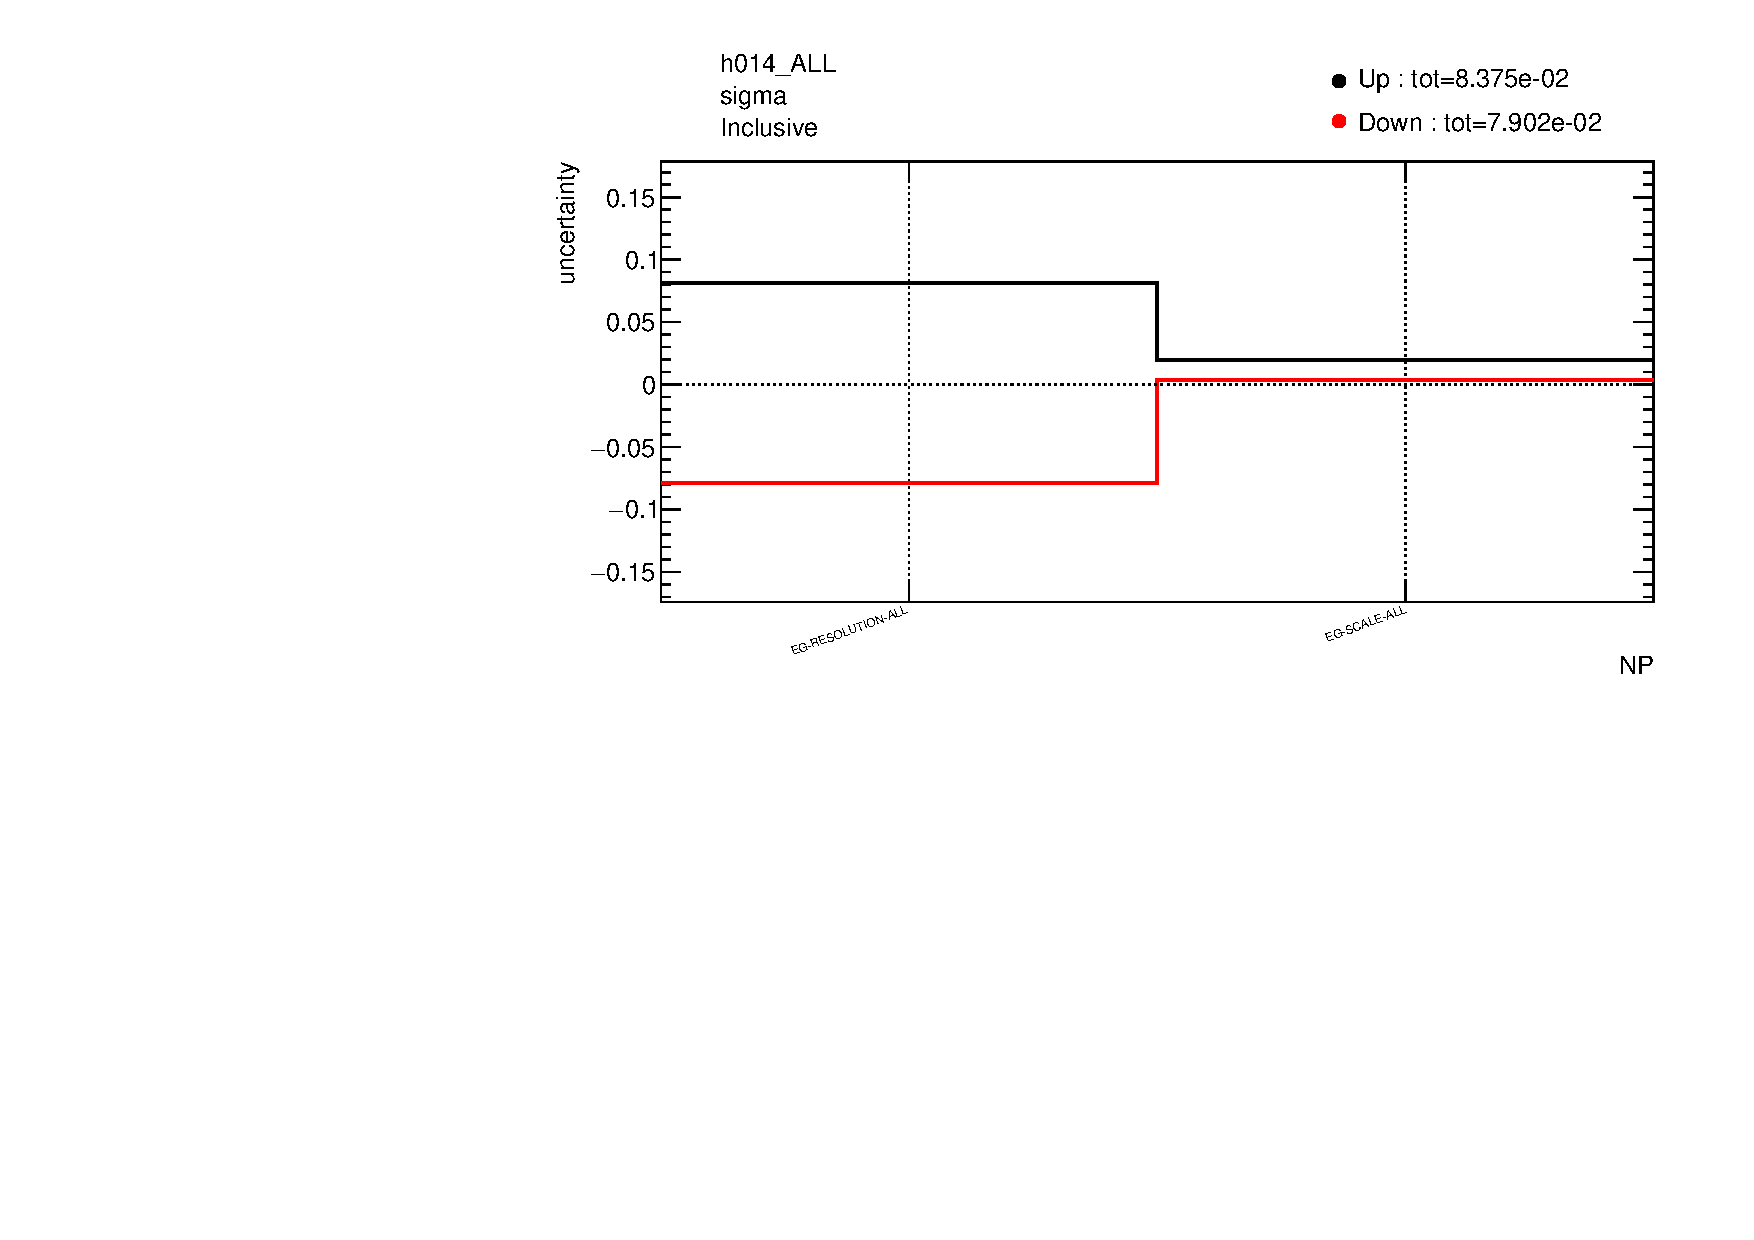
\includegraphics[width=\linewidth]{./plots/h014_ALL_Systematics_Inclusive_sigma_sigma.pdf}
\end{center}
\end{column}

\begin{column}{0.5\columnwidth}
\begin{center}
\includegraphics[width=\linewidth]{/home/goudet/Documents/LAL/Zim/Hgam/PhotonSystematic/170209_CompareSystModel_h014.pdf}
\end{center}
\end{column}
\end{columns}
\end{frame}
\end{document}